% !TeX spellcheck = en_US

% We need layers to draw the block diagram
\usetikzlibrary{calc,positioning}
\usetikzlibrary{arrows.meta}

% Define a few styles and constants
\tikzstyle{entry}=[draw, fill=green!20, minimum height=2.5em, align=center]
\tikzstyle{text} = [above, text width=5em]
\tikzstyle{topology} = [entry, text width=18em, fill=white, 
minimum height=28em, rounded corners]
\tikzstyle{rtemplate} = [entry, text width=7em, shading = axis,rectangle, left color=blue!10!white, right color=blue!30!white,shading angle=135, anchor=north,
minimum height=10em, rounded corners]
\tikzstyle{item} = [entry, text width=5em, shading = axis,rectangle, left color=blue!10!white, right color=blue!30!white,shading angle=135, anchor=north,
minimum height=1.5em, rounded corners]
\tikzstyle{ntemplate} = [entry, text width=7em, shading = axis,rectangle, left color=blue!10!white, right color=blue!30!white,shading angle=135, anchor=north,
minimum height=8em, rounded corners]
\tikzstyle{rtype} = [entry, text width=6.5em, shading = axis,rectangle, left color=blue!10!white, right color=blue!30!white,shading angle=135, anchor=north,
minimum height=4em, rounded corners]
\tikzstyle{ntype} = [entry, text width=6.5em, shading = axis,rectangle, left color=blue!10!white, right color=blue!30!white,shading angle=135, anchor=north,
minimum height=7em, rounded corners]
\def\blockdist{2.3}
\def\edgedist{2.5}

\begin{figure}
	\centering
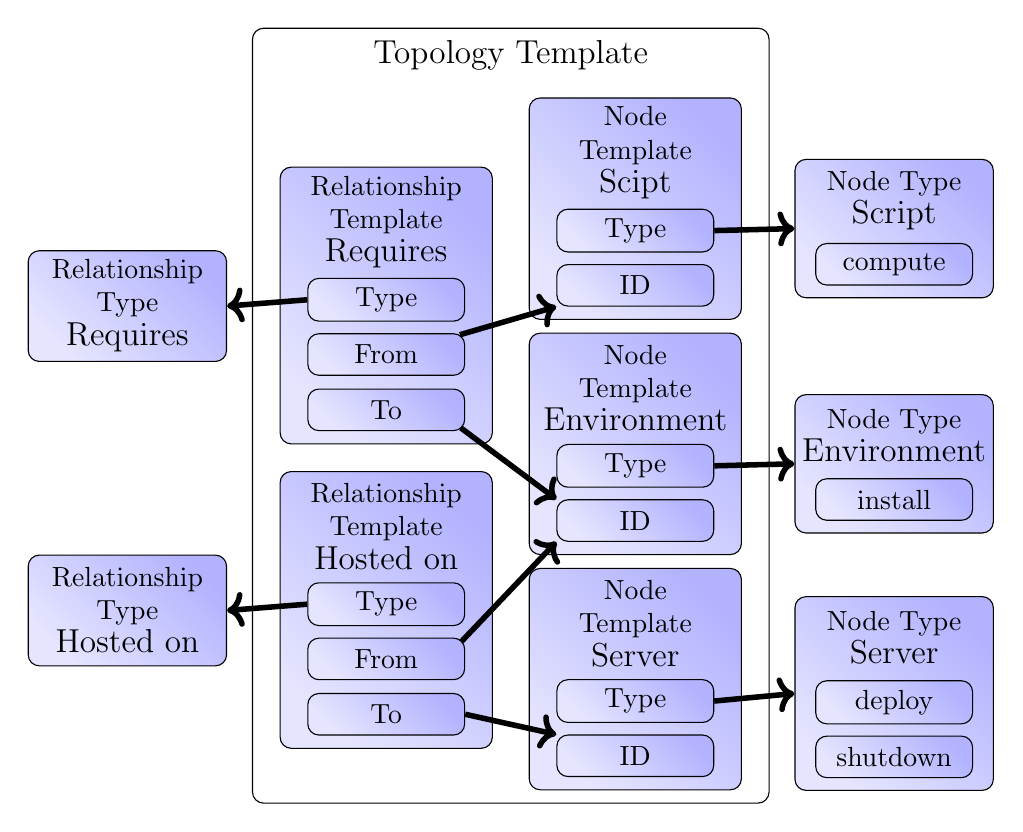
\begin{tikzpicture}
\node (topology) [topology] {};
\node at (topology.north)[yshift=-1em] {\large Topology Template};


\node (requirestemplate) [xshift=-4.5em, yshift=+9em] at ( topology) [rtemplate] {};
\node (requirestemplatetype) at (requirestemplate) [yshift=+1em] [item] {Type};
\node (requirestemplatefrom) at (requirestemplate) [yshift=-1em] [item] {From};
\node (requirestemplateto) at (requirestemplate) [yshift=-3em] [item] {To};
\node at (requirestemplate.north) [yshift=-2em][align=center] {Relationship\\Template\\\large Requires};

\node (hostedtemplate) [xshift=-4.5em, yshift=-2em] at ( topology) [rtemplate] {};
\node (hostedtemplatetype) at (hostedtemplate) [yshift=+1em] [item] {Type};
\node (hostedtemplatefrom) at (hostedtemplate) [yshift=-1em] [item] {From};
\node (hostedtemplateto) at (hostedtemplate) [yshift=-3em] [item] {To};
\node at (hostedtemplate.north) [yshift=-2em][align=center] {Relationship\\Template\\\large Hosted on};

\node (scripttemplate) [xshift=+4.5em, yshift=+11.5em] at ( topology) [ntemplate] {};
\node (scripttemplatetype) at (scripttemplate) [yshift=+0em] [item] {Type};
\node (scripttemplateID) at (scripttemplate) [yshift=-2em] [item] {ID};
\node at (scripttemplate.north) [yshift=-2em][align=center] {Node\\Template\\\large Scipt};

\node (environmenttemplate) [xshift=+4.5em, yshift=+3em] at ( topology) [ntemplate] {};
\node (environmenttemplatetype) at (environmenttemplate) [yshift=+0em] [item] {Type};
\node (environmenttemplateID) at (environmenttemplate) [yshift=-2em] [item] {ID};
\node at (environmenttemplate.north) [yshift=-2em][align=center] {Node\\Template\\\large Environment};

\node (servertemplate) [xshift=+4.5em, yshift=-5.5em] at ( topology) [ntemplate] {};
\node (servertemplatetype) at (servertemplate) [yshift=+0em] [item] {Type};
\node (servertemplateID) at (servertemplate) [yshift=-2em] [item] {ID};
\node at (servertemplate.north) [yshift=-2em][align=center] {Node\\Template\\\large Server};

\node (requirestype) [xshift=-5.5em, yshift=+2em] at ( requirestemplate.west) [rtype] {};
\node at (requirestype.north) [yshift=-2em][align=center] {Relationship\\Type\\\large Requires};

\node (hostedontype) [xshift=-5.5em, yshift=+2em] at ( hostedtemplate.west) [rtype] {};
\node at (hostedontype.north) [yshift=-2em][align=center] {Relationship\\Type\\\large Hosted on};

\node (scripttype) [xshift=+5.5em, yshift=+1.8em] at ( scripttemplate.east) [ntype, minimum height=5em] {};
\node  at (scripttype.south) [yshift=+2em] [item] {compute};
\node at (scripttype.north) [yshift=-1.5em][align=center] {Node Type\\\large Script};

\node (environmenttype) [xshift=+5.5em, yshift=+1.8em] at ( environmenttemplate.east) [ntype, minimum height=5em] {};
\node  at (environmenttype.south) [yshift=+2em] [item] {install};
\node at (environmenttype.north) [yshift=-1.5em][align=center] { Node Type\\\large Environment};

\node (servertype) [xshift=+5.5em, yshift=+3em] at ( servertemplate.east) [ntype] {};
\node  at (servertype.south) [yshift=+4em] [item] {deploy};
\node  at (servertype.south) [yshift=+2em] [item] {shutdown};
\node at (servertype.north) [yshift=-1.5em][align=center] { Node Type\\\large Server};

\draw [->,scale=5,line width=2pt,shorten <= -2pt] (requirestemplatefrom.north east) -- (scripttemplateID.south west);
\draw [->,scale=5,line width=2pt,shorten <= -2pt] (requirestemplateto.south east) -- (environmenttemplateID.north west);
\draw [->,scale=5,line width=2pt,shorten <= -2pt] (hostedtemplatefrom.north east) -- (environmenttemplateID.south west);
\draw [->,scale=5,line width=2pt] (hostedtemplateto.east) -- (servertemplateID.north west);

\draw [->,scale=5,line width=2pt] (requirestemplatetype.west) -- (requirestype.east);
\draw [->,scale=5,line width=2pt] (hostedtemplatetype.west) -- (hostedontype.east);

\draw [->,scale=5,line width=2pt] (servertemplatetype.east) -- (servertype.west);
\draw [->,scale=5,line width=2pt] (environmenttemplatetype.east) -- (environmenttype.west);
\draw [->,scale=5,line width=2pt] (scripttemplatetype.east) -- (scripttype.west);
\end{tikzpicture} 
\caption{Example: a cloud application for weather calculation} 	\label{fig:weather}
\end{figure}